%% this is necessary stuff to make the document compile:
\documentclass[reqno,11pt]{article}
\usepackage{amssymb, amsmath}
\usepackage{colordvi,verbatim,hyperref}
\usepackage{graphicx}
\usepackage{amsthm}

\usepackage[dvipsnames]{xcolor}
\usepackage{tikz}
\usetikzlibrary{positioning}
\usetikzlibrary{snakes}

%% this is for making margins the way I like them:
\headheight=8pt
\topmargin=0.375truein
\topmargin=-0.2truein
\textheight=9truein   \textwidth=6.3truein
\oddsidemargin=.1in \evensidemargin=.1in

%%this is to create new math commands. In other words, since I use theta^hat in equations a lot, I made a shorthand for it. So now instead of using $\hat\theta$ every time, I can just write $\thhat$. 
\newcommand{\Q}{{\mathbb{Q}}}
\newcommand{\N}{{\mathbb{N}}}
\newcommand{\R}{{\mathbb{R}}}
\newcommand{\rhs}{{\text{RHS}}}

\pagestyle{plain}


\date{\today}%7 Feb 2014}

\begin{document}
\title{An Analogy of Approximation Methods}
\author{Trenton Gerew}

\maketitle
	\begin{figure}[h!]
		\centering
		
		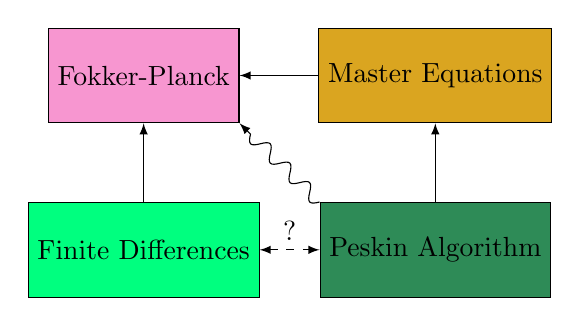
\begin{tikzpicture}
			% F-P
			\node [draw,
				fill=Rhodamine!50,
				minimum width=2cm,
				minimum height=1.2cm
				] (fp) at (0,0) {Fokker-Planck};
			
			% Master Equations
			\node [draw,
				fill=Goldenrod,
				minimum width=2cm,
				minimum height=1.2cm,
				right=1cm of fp
				] (me) {Master Equations};
				
			% Finite Differences
			\node [draw,
				fill=SpringGreen,
				minimum width=2cm,
				minimum height=1.2cm,
				below=1cm of fp
				] (fd) {Finite Differences};
				
			% Peskin Algorithm
			\node [draw,
				fill=SeaGreen,
				minimum width=2cm,
				minimum height=1.2cm,
				below=1cm of me
				] (pa) {Peskin Algorithm};
				
			% Arrows
			\draw[-latex] (me.west) -- (fp.east);
			\draw[-latex] (fd.north) -- (fp.south);
			\draw[-latex] (pa.north) -- (me.south);
			\draw[-latex,snake=coil,segment aspect=0] (pa.north west) -- (fp.south east);
			\draw[latex-latex,dashed] (fd.east) -- (pa.west)
				node[midway,above]{?};
		
		\end{tikzpicture}
		
		\caption{Approximation methods and their relationships to the Fokker-Planck equation. \label{fig:relationships}}
	\end{figure}

	The probability density $u (x,t)$ evolves according to the Fokker-Planck equation
	\begin{equation}
		\label{eq:f-p}
		\partial_t u (x,t) = \partial_x \left( u (x,t) \phi' (x) + \partial_x u (x,t) \right)
	\end{equation}
	where $\phi (x)$ is the potential energy \cite{WANG2003491}.
	In one spatial dimension, this is a simple convection-diffusion equation.
	
	\section{Finite Differences}
	First we will write an explicit finite difference scheme for \eqref{eq:f-p}.
	We assume we work on the closed domain $[0,1] \times [0,t_F]$.
	Note that we must use a finite time interval, but $t_F$ can be made as large as desired.
	We denote the uniform spacings by $h$ and $s$ for space and time, respectively.
	Then the mesh points are
	\begin{equation*}
		(x_j = j h, t_n = n s), \ j = 0,1,2\dots,J, \ n = 0,1,2,\dots,
	\end{equation*}
	and $h = 1 / J$.
	We use the notation
	\begin{equation*}
		U_j^n \approx u (x_j,t_n)
	\end{equation*}
	to mean the approximations of the solution at the mesh points.
	
	The left side of \eqref{eq:f-p} is approximated using a forward difference for the time derivative:
	\begin{equation}
		\label{eq:t-fd}
		\frac{U_j^{n+1} - U_j^n}{s} \approx \frac{\partial u (x_j,t_n)}{\partial t}.
	\end{equation}
	
	Next will we derive the approximation for the right side of \eqref{eq:f-p}.
	We rewrite this as
	\begin{equation*}
		\partial_x (u \phi') + u_{xx} = \partial_x (u \phi' + u_x).
	\end{equation*}
	Rather than expanding the first term using the product rule, we follow \cite{morton_mayers_2005} and write
	\begin{equation*}
		U_{j+1/2}^n \left( \frac{ \phi_{j+1} - \phi_j}{h} \right) \approx \left[ u (x,t) \frac{d \phi (x)}{dx} \right]_{j+1/2}^n
	\end{equation*}
	and similarly for $j$ replaced with $j-1$.
	Subtracting these two and dividing by $h$, we obtain
	\begin{equation*}
		\frac{1}{h^2} \left[ U_{j+1/2}^n \Delta_j \phi - U_{j-1/2}^n \Delta_{j-1} \phi \right] \approx \partial_x \left( u (x_j,t_n) \phi' (x_j) \right)
	\end{equation*}
	where $\Delta_j \phi = \phi_{j+1} - \phi_j$ and $\Delta_{j-1} \phi = \phi_j - \phi_{j-1}$.
	This approach requires the computation of $u (x,t)$ for values of $x$ half-way between space steps.
	An alternative is to use
	\begin{equation*}
		\frac{1}{2} \left( U_{j+1}^n + U_j^n \right) \approx U_{j+1/2}^n
	\end{equation*}
	and similarly for $j$ replaced with $j-1$.
	Making these approximations, we arrive at
	\begin{equation}
		\label{eq:s1-fd}
		\frac{1}{2 h^2} \left[ ( U_{j+1}^n + U_j^n ) \Delta_j \phi + ( U_j^n + U_{j-1}^n ) \Delta_{j-1} \phi \right] \approx \partial_x (u \phi').
	\end{equation}
	For the second term of the right side, we use a centered second difference:
	\begin{equation}
		\label{eq:s2-fd}
		\frac{1}{h^2} \left[ U_{j+1}^n - 2 U_j^n + U_{j-1}^n \right] \approx u_{xx}.
	\end{equation}
	Now adding \eqref{eq:s1-fd} and \eqref{eq:s2-fd} we obtain the full approximation for the right side of \eqref{eq:f-p}.
	Since this scheme is explicit, we can solve for $U_j^{n+1}$ easily:
	\begin{equation}
		\label{eq:fd-scheme}
		U_j^{n+1} = U_j^n + \frac{s}{2 h^2} \left[ U_{j+1}^n ( \Delta_j \phi + 2 ) + U_j^n ( \Delta_j \phi + \Delta_{j-1} \phi - 4 ) + U_{j-1}^n ( \Delta_{j-1} \phi + 2 ) \right]
	\end{equation}
	
	\section{Master Equations}
		We now try to derive the same set of equations by considering a spatially discrete jump process.
		At any spacial point $j$, the change in the probability of that point being occupied in time can be described as \textit{Flux In} - \textit{Flux Out}.
		Using $F_{j+1/2}$ to denote the forward jump from $x_j$ to $x_{j+1}$ and $B_{j+1/2}$ to denote a backward jump from $x_{j+1}$ to $x_j$, we can write
		\begin{equation}
			\label{eq:markov}
			\frac{d U_j}{dt} = \left[ F_{j-1/2} U_{j-1} + B_{j+1/2} U_{j+1} \right] - \left[ F_{j+1/2} U_j + B_{j-1/2} U_j \right].
		\end{equation}
		We define $F_{j+1/2}$ and $B_{j+1/2}$ according to \cite{morton_mayers_2005}:
		\begin{equation*}
			\begin{aligned}
				F_{j+1/2} &= \frac{1}{h^2} \frac{\Delta_j \phi}{\exp ( \Delta_j \phi ) - 1}, \\
				B_{j+1/2} &= \frac{1}{h^2} \frac{- \Delta_j \phi}{\exp ( - \Delta_j \phi ) - 1}.
			\end{aligned}
		\end{equation*}
		We can compute the Taylor expansion of these to find
		\begin{equation}
			\label{eq:jumps}
			\begin{aligned}
				F_{j+1/2} &\approx \frac{1 - \Delta_j \phi / 2 + O \left( ( \Delta_j \phi )^2 \right)}{h^2}, \\
				B_{j+1/2} &\approx \frac{1 + \Delta_j \phi / 2 + O \left( ( \Delta_j \phi )^2 \right)}{h^2}.
			\end{aligned}
		\end{equation}
		Now substituting \eqref{eq:jumps} into \eqref{eq:markov}, we find
		%\begin{equation}
			
		
	
	\bibliographystyle{abbrv}
	\bibliography{methods}
\end{document}